%package list
\documentclass{article}
\usepackage[english,spanish]{babel}
\usepackage[utf8]{inputenc}
\usepackage[top=3cm, bottom=3cm, outer=3cm, inner=3cm]{geometry}
\usepackage{multicol}
\usepackage{graphicx}
\usepackage{url}
\usepackage{hyperref}
\usepackage{array}
\newcolumntype{x}[1]{>{\centering\arraybackslash\hspace{0pt}}p{#1}}
\usepackage{natbib}
\usepackage{pdfpages}
\usepackage{multirow}
\usepackage[normalem]{ulem}
\useunder{\uline}{\ul}{}
\usepackage{svg}
\usepackage{xcolor}
\usepackage{listings}
\usepackage{caption}
\usepackage{subcaption}
\usepackage{float}
\usepackage{array}
\usepackage[english,spanish]{babel}
\usepackage[utf8]{inputenc}
\usepackage{fancyhdr}
\usepackage{listings}
\usepackage{color, colortbl}
\usepackage{amsmath}

\lstdefinestyle{ascii-tree}{
    literate={├}{|}1 {─}{--}1 {└}{+}1 
  }
  
\lstset{basicstyle=\ttfamily,
  showstringspaces=false,
  commentstyle=\color{red},
  keywordstyle=\color{blue}
}

\newcolumntype{M}[1]{>{\centering\arraybackslash}m{#1}}
\newcolumntype{N}{@{}m{0pt}@{}}

%%%%%%%%%%%%%%%%%%%%%%%%  ITEMS  %%%%%%%%%%%%%%%%%%%%%%%%%%%%%%%%%

\newcommand{\itemUniversity}{Universidad Nacional de San Agustín de Arequipa}
\newcommand{\itemFaculty}{Facultad de Ingeniería de Producción y Servicios}
\newcommand{\itemSchool}{Escuela Profesional de Ingeniería de Sistemas}
\newcommand{\itemCourse}{Estructura de datos y Algoritmos}
\newcommand{\itemTheme}{Técnicas de Diseño de Algoritmos}

%%%%%%%%%%%%%%%%%%%%%%%%   HEADER   %%%%%%%%%%%%%%%%%%%%%%%%%%%%%%

\AtBeginDocument{\selectlanguage{spanish}}
\renewcommand{\figurename}{Figura}
\renewcommand{\refname}{Referencias}
\renewcommand{\tablename}{Tabla} 
\AtBeginDocument{%
	\renewcommand\tablename{Tabla}
}

\pagestyle{fancy}
\fancyhf{}
\setlength{\headheight}{30pt}
\renewcommand{\headrulewidth}{1pt}
\renewcommand{\footrulewidth}{1pt}

\fancyhead[L]{\raisebox{-0.2\height}{
\includegraphics[width=3cm]{img/logo_episunsa.png}}}
\fancyhead[C]{\fontsize{7}{7}\selectfont	\itemUniversity \\ \itemFaculty \\ \itemDepartment \\ \itemSchool \\ \textbf{\itemCourse}}
\fancyhead[R]{\raisebox{-0.2\height}{
\includegraphics[width=1.2cm]{img/logo_abet}}}

\fancyfoot[L]{Reyser Z. - Jhastyn P.}
\fancyfoot[C]{\itemCourse}
\fancyfoot[R]{Página \thepage}

% para el codigo fuente
\definecolor{dkgreen}{rgb}{0,0.6,0}
\definecolor{gray}{rgb}{0.5,0.5,0.5}
\definecolor{mauve}{rgb}{0.58,0,0.82}
\definecolor{codebackground}{rgb}{89, 0.97, 0.90}
\definecolor{tablebackground}{rgb}{0.8, 0, 0}

\lstset{frame=tb,
	language=bash,
	aboveskip=3mm,
	belowskip=3mm,
	showstringspaces=false,
	columns=flexible,
	basicstyle={\small\ttfamily},
	numbers=none,
	numberstyle=\tiny\color{gray},
	keywordstyle=\color{blue},
	commentstyle=\color{dkgreen},
	stringstyle=\color{mauve},
	breaklines=true,
	breakatwhitespace=true,
	tabsize=3,
	backgroundcolor= \color{codebackground},
}

%%%%%%%%%%%%%%%%%%%%%%   CARATULA  %%%%%%%%%%%%%%%%%%%%%%%%%%%%%%%%%
\begin{document} 
    \begin{titlepage}
    \centering
    
    {\bfseries\LARGE {\itemUniversity} \par} \vspace{0.3 cm}
    {\scshape\Large {\itemFaculty} \par} \vspace{0.3 cm}
    {\scshape\Large {\itemSchool} \par}\vspace{1 cm}

    {
\includegraphics[width=0.4\textwidth]{{img/logo_unsa_corto.png}}\par}
    \vspace{0.5 cm}
    
    {\scshape\LARGE  INFORME DE TRABAJO GRUPAL \par}
    {\scshape\Large {\itemCourse} \par}
    \vspace{1 cm}
    
    {\Large Alumnos:\par}
    {\begin{itemize} \centering 
        \item {\Large Payehuanca Riquelme Jhastyn Jefferson\par}
        \item {\Large Zapata Butron Reyser Julio\par}
    \end{itemize}}
    \vspace{0.5 cm}
    
    {\Large Docente:\par}
    {\Large Quispe Vergaray Karen Melissa\par}
    \vfill
    \vspace{1 cm}
    
    {\Large 30 de septiembre 2023 \par}
    {\Large Arequipa - Perú \par}
    
    \end{titlepage}
%%%%%%%%%%%%%%%%%%%%%%   CONTENIDO   %%%%%%%%%%%%%%%%%%%%%%%%%%%%%%%%%
 
    \vspace*{2px}
	
    \begin{center}	
        \fontsize{17}{17} \textbf{Informe Trabajo Grupal}
    \end{center}
 
    \centerline{\textbf{\Large Tema: \itemTheme}}

%%%%%%%   REPOSITORIO   %%%%%%% 
    \section{URL de Repositorio Github}
        \textbf{Link del Repositorio en Github: }    
            \url{https://github.com/ReyserLyn/eda-lab2.git}

%%%%%%%   EJERCICIOS   %%%%%%%     
	
    \section{Ejercicios designados}

    \begin{itemize}
        \item Fibonacci recursivo
        \item Fibonacci iterativo
        \item Fibonacci con memorización no iterativo
        \item Fibonacci logaritmico
        \item Informe sobre prueba realizadas para valores n grandes (1000, 10000, 1000000 ...)
    \end{itemize}

 %%%%%%%   SOLUCIÓN   %%%%%%%     
    \section{Solución}
    
        \textbf{Explicación de la función Main}\par  
            \begin{itemize}
                \item {El programa comienza por procesar los argumentos de la línea de comandos, donde args[0] se interpreta como el número para el cual se calculará el valor de Fibonacci y args[1] sería una indicación si mostrar el numero resultante o no.}
                \item {Se registra el tiempo de inicio (tmpInicio) antes de realizar el cálculo.}
                \item {Luego, se calcula el valor de Fibonacci llamando a la función fibonacci\_iterativo(x).}
                \item {Se registra el tiempo de finalización (tmpFin) después de calcular el valor de Fibonacci y se calcula el tiempo transcurrido en milisegundos (tmpTrans).}
                \item {Si el segundo argumento (args[1]) proporcionado es "true", el programa imprime el resultado de Fibonacci.}
                \item {Finalmente, se imprime el tiempo de ejecución en milisegundos.}
            \end{itemize}
            
        \subsection{Fibonacci Recursivo}
            Para la implementación recursiva de la secuencia de Fibonacci se calcula mediante llamadas a funciones recursivas. En este enfoque, el número de Fibonacci en un índice n dado se calcula sumando recursivamente los números de Fibonacci en los índices n-1 y n-2, con casos base definidos para n=0 y n=1.

            \lstinputlisting[language=Java, caption={Fib\_Recursivo.java},numbers=left,]{src/Fib_Recursivo.java}

            \textbf{Explicación de la función fibonacci\_recursivo}\par  
            \begin{itemize}
                \item If \(n \leq 1\), then return \(\text{BigInteger.valueOf}(n)\): Si \(n\) es menor o igual a 1 (es decir, es un caso base), este método devuelve \(\text{BigInteger.valueOf}(n)\), que es 0 o 1, dependiendo del valor de \(n\).
                \item Otherwise, return \(\text{fibonacci\_recursivo}(n - 1) + \text{fibonacci\_recursivo}(n - 2)\): Si \(n\) es mayor que 1 (es decir, no es un caso base), el método calcula el número de Fibonacci de forma recursiva llamándose a sí mismo con \(n - 1\) y \(n - 2\), y luego sumando los resultados. Este enfoque recursivo continúa hasta llegar a los casos base.
            \end{itemize}
        
        \subsection{Fibonacci Iterativo}
            Para la implementación iterativa de Fibonacci se utliza un bucle para calcular los números de la secuencia en orden ascendente. Es eficiente y evita los problemas de desbordamiento de pila que pueden ocurrir con la implementación recursiva cuando se calculan números grandes. En esta implementación, se utiliza el tipo de dato BigInteger para manejar números grandes que puedan generarse en la secuencia de Fibonacci.
            
            \lstinputlisting[language=Java, caption={Fib\_Iterativo.java},numbers=left,]{src/Fib_Iterativo.java}	         
            
            \textbf{Explicación de la función fibonacci\_iterativo}\par  
            \begin{itemize}
                \item {Se manejan los casos base para 0 y 1. Si num es igual o menor a 1, se devuelve el valor correspondiente (0 o 1) como un objeto BigInteger.}
                \item {Dentro del bucle for, se calcula el valor de Fibonacci iterativamente utilizando tres objetos BigInteger: fibPrevPrev, fibPrev, y fibCurrent.}
                \item {Los valores anteriores se actualizan en cada iteración para calcular el siguiente valor de Fibonacci.}
                \item {Al final, se devuelve el valor calculado como un objeto BigInteger.}
            \end{itemize}
        
        \subsection{Fibonacci con Memorización no Iterativo}
            Para la implementación con memorización no iterativo de Fibonacci utilizamos un mapa de memorización que nos servirá para almacenar los números de Fibonacci que ya han sido calculados, lo que ayuda a evitar cálculos redundantes y mejora la eficiencia del algoritmo.            
            Este enfoque es más eficiente que el enfoque puramente recursivo para calcular los números de Fibonacci, especialmente para valores más grandes de n, porque evita recalcular los mismos números de Fibonacci varias veces.

            \lstinputlisting[language=Java, caption={Fib\_Memorizacion.java},numbers=left,]{src/Fib_Memorizacion_no_Iterativo.java}

            \textbf{Explicación de la función fibonacci\_memorizacion}
            \begin{itemize}
                \item Es una función que calcula el número de Fibonacci para un índice dado \(n\) utilizando el enfoque de memorización (memoization).
                \item La primera parte de la función. Verifica si \(n\) es menor o igual a 1. Si es así, significa que \(n\) es un caso base de la secuencia de Fibonacci, y simplemente devuelve \(n\) convertido en un objeto \texttt{BigInteger} utilizando \texttt{BigInteger.valueOf}(n). En este caso, el resultado será 0 para \(n=0\) y 1 para \(n=1\).
                \item La segunda parte de la función. Si \(n\) no es un caso base (es decir, \(n\) es mayor que 1), verifica si el resultado para \(n\) ya está almacenado en el mapa de memorización (\texttt{memo}). Si el resultado ya está en el mapa, lo recupera utilizando \texttt{memo.get}(n) y lo devuelve. Esto evita calcular el mismo número de Fibonacci más de una vez y mejora la eficiencia del algoritmo.
                \item La tercera parte de la función. Si \(n\) no es un caso base y el resultado no está en el mapa de memorización, se calcula el número de Fibonacci para \(n\) de manera recursiva. Esto se hace llamando a \texttt{fibonacci\_memorizacion}(n - 1) para obtener el número de Fibonacci para \(n - 1\) y \texttt{fibonacci\_memorizacion}(n - 2) para obtener el número de Fibonacci para \(n - 2\). Luego, se suman estos dos resultados para obtener el número de Fibonacci para \(n\). El resultado se almacena en el mapa de memorización (\texttt{memo.put}(n, result)) para futuras referencias y se devuelve como un objeto \texttt{BigInteger}.
            \end{itemize}
        
        \subsection{Fibonacci Logaritmico}
            Para la implementación logarítmica de Fibonacci se utiliza la técnica de "exponenciación rápida". Esta estrategia eficiente permite calcular los números de Fibonacci en tiempo logarítmico en lugar de un enfoque lineal. La clave de esta eficiencia reside en el uso de matrices y la reducción de operaciones redundantes. Además, esta técnica es especialmente beneficiosa cuando se trabaja con números grandes de la secuencia de Fibonacci, ya que evita el desbordamiento de valores y mejora significativamente el rendimiento en comparación con la implementación recursiva o iterativa estándar.

            \lstinputlisting[language=Java, caption={Fib\_logaritmico.java},numbers=left,]{src/Fib_logaritmico.java}	

            \textbf{Explicación de la función fibonacci\_logaritmico}\par  
            \begin{itemize}
                \item {La función fibonacci\_logaritmico calcula el valor de Fibonacci de manera logarítmica utilizando la técnica de exponentiación rápida.}
                \item {Si n es menor o igual a 0, se devuelve 0 como un objeto BigInteger (caso base).}
                \item {Se crea una matriz matriz inicializada con valores iniciales {{1, 1}, {1, 0}}, que se utiliza para realizar la exponentiación rápida.}
                \item {Se llama a la función elevarMatriz para elevar la matriz a la potencia n - 1. El resultado se encuentra en matriz[0][0] y representa el valor de Fibonacci deseado.}
            \end{itemize}

            \textbf{Explicación de la función multiplicarMatriz}\par  
            \begin{itemize}
                \item {La función multiplicarMatriz implementa la multiplicación de dos matrices cuadradas A y B y actualiza la matriz A con el resultado. Este es un paso fundamental en la técnica de exponentiación rápida.}
            \end{itemize}

            \textbf{Explicación de la función elevar\_matriz}\par  
            \begin{itemize}
                \item {La función elevarMatriz implementa la técnica de exponentiación rápida para elevar la matriz matriz a la potencia n.}
                \item {La recursión se utiliza para dividir el problema en subproblemas más pequeños.}
                \item {Se llama a elevarMatriz(matriz, n \// 2) para calcular matriz\^(n\//2) y luego se multiplica matriz por sí misma utilizando multiplicarMatriz(matriz, matriz).}
                \item {Si n es impar (n \% 2 != 0), se multiplica matriz por base para tener en cuenta el término adicional.}
            \end{itemize}
        
        \subsection{Pruebas de Eficiencia}
            \subsubsection{Recursiva}
            \begin{center}
                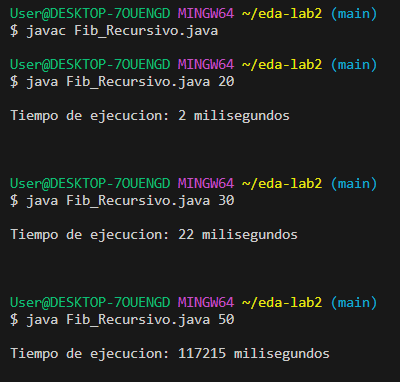
\includegraphics[width=0.8\textwidth]{img/tmp_recursivo.png}
            \end{center}
            Como pueden ver el tiempo de ejecución es bastante para tan solo 50 números, por lo tanto no es recomendable utilizar el método recursivo, ya que al momento de su ejecución es muy redundante.
            
            \subsubsection{Iterativo}
            \begin{center}
                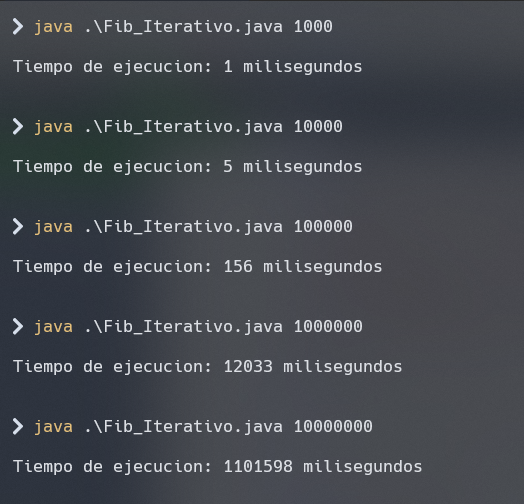
\includegraphics[width=0.8\textwidth]{img/tmp_iterativo.png}
            \end{center}
            Como se puede observar en la anterior imagen, para calcular el número 10 millones en la serie de Fibonacci se demoró 18 minutos aprox. 

            \subsubsection{Memorización no iterativa}
            \begin{center}
                \includegraphics[width=0.8\textwidth]{img/tmp_memorización.png}
            \end{center}
            Es más eficiente que el recursivo de por si ya que este almacena valores y omite calculos ya redundantes, pero aún así no es la mejor alternativa.
            
            \subsubsection{Logaritmica}
            \begin{center}
                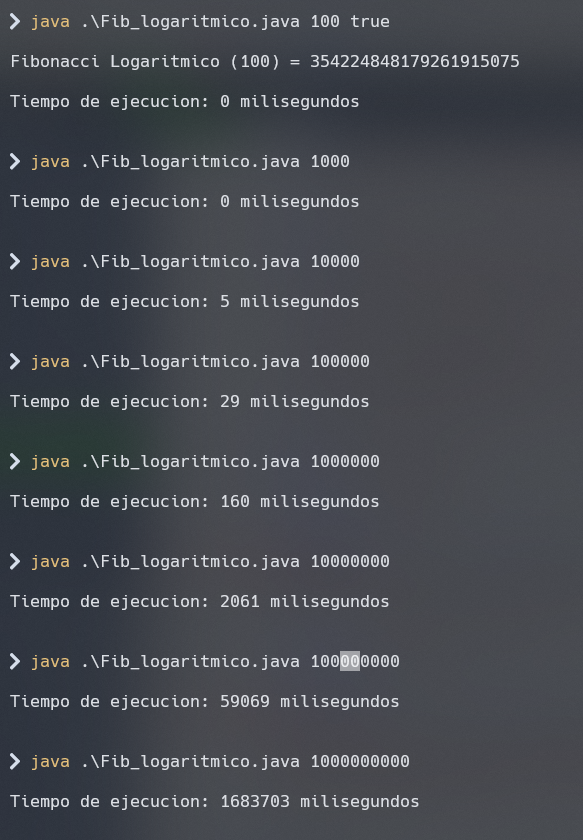
\includegraphics[width=0.8\textwidth]{img/tmp_logaritmica.png}
            \end{center}
            Como se puede observar en la anterior imagen, este método es muy eficiente, el mejor de los que se presentaron, pudiendo calcular el número \textbf{1 BILLÓN} en un tiempo de 28 minutos aprox. Mientras que el número 100 MILLONES en un tiempo de 1 minutos. 

 %%%%%%%   CONCLUSIONES   %%%%%%%     

    \section{Conclusiones}
        \begin{itemize}
            \item {El enfoque recursivo es útil para comprender la naturaleza de la secuencia de Fibonacci, pero no es eficiente para cálculos prácticos de números grandes. Por otro lado, el enfoque con memorización es altamente eficiente y es la opción preferida cuando se requieren cálculos precisos y rápidos de la secuencia de Fibonacci, incluso para números grandes. }
            \item {La implementación de la secuencia de Fibonacci utilizando la técnica de "exponentiación rápida" es una estrategia altamente eficiente, especialmente cuando se trabaja con números grandes. Este enfoque logarítmico reduce significativamente el tiempo de cálculo y evita problemas de desbordamiento de valores, lo que lo convierte en una opción poderosa para calcular la secuencia de Fibonacci en escenarios donde la eficiencia es esencial.}
        \end{itemize}
        
%%%%%%%   REFERENCIAS   %%%%%%% 
    \section{Referencias}
    
    \begin{itemize}			
    	\item \url{https://www.cs.us.es/~jalonso/cursos/i1m-15/temas/tema-24.html}
    	\item \url{https://dev.java/learn/}
    	\item \url{https://www.ugr.es/~eaznar/fibo.htm}     
    \end{itemize}	

%%%%%%%   END   %%%%%%% 
\end{document}